\ifdefined\COMPILINGFROMMAIN
\else
    %%%%HEADER
\documentclass[twocolumn]{article}
\usepackage[a4paper, margin=1in, columnsep=20pt]{geometry}
\usepackage{amsmath, amssymb, graphicx, hyperref}
\usepackage[most,skins,breakable]{tcolorbox}
\usepackage[symbol]{footmisc}
\usetikzlibrary{calc}
\usepackage{xcolor}
\usepackage{caption}
\usepackage{algorithm}
\usepackage{algpseudocodex}
\usepackage{tikz}
\usepackage{listings}
\usetikzlibrary{arrows.meta, positioning}
\tcbuselibrary{listingsutf8}
\usepackage{microtype}
\usepackage{blindtext}
\usepackage{bookmark}
\usepackage{breqn}
\usepackage[backend=biber,style=numeric]{biblatex} % 
\addbibresource{../references.bib}

% Define style for the listings environment
\lstdefinestyle{mystyle}{
    basicstyle=\ttfamily\small,
    breaklines=true,
    escapeinside={(*@}{@*)}, % Allows math mode within listings
    numbers=left,
    numberstyle=\tiny,
    frame=single,
    keywordstyle=\color{blue}\bfseries,
    commentstyle=\color{green!50!black},
    stringstyle=\color{red}
}


\def\reals{\mathbb{R}}
% Define the custom definition box and command
\newtcolorbox{mydefinition}[2][]{%
    text width=0.95\columnwidth,
    before=\vspace{1mm}, 
    after=\vspace{1mm}, 
    colback=gray!10, % Background color (light gray)
    colframe=black!70,  % Border color
    coltitle=gray!10,  % Title color
    fonttitle=\bfseries, % Title font style
    sharp corners,   % Box style
    left=2pt,
    breakable,
    right=2pt,
    top=2pt,
    bottom=2pt,
    enhanced jigsaw,
    title=Definition: {#1},         % Title passed as the first argument
    colupper=black,  % Ensure proper content handling
    pad at break*=1pc,
    overlay first and middle={
        \coordinate (A1) at ($(interior.south east) + (-10pt,5pt)$);
        \coordinate (C1) at ($(interior.south east) + (-6pt,7.5pt)$);
        \draw[fill=black!50] (A1) -- +(0,5pt) -- (C1) -- cycle;
    }
    }
    
\newcommand{\definition}[2]{%
    \noindent%
    \begin{mydefinition}[#1]%
        .#2%
    \end{mydefinition}%
    \noindent
}

\newtcolorbox{myexample}[2][]{%
    text width=0.95\columnwidth,
    before=\vspace{1mm}, 
    after=\vspace{1mm}, 
    colback=orange!3, % Background color (light gray)
    colframe=black!70,  % Border color
    coltitle=gray!10,  % Title color
    fonttitle=\bfseries, % Title font style
    sharp corners,   % Box style
    left=2pt,
    right=2pt,
    top=2pt,
    bottom=2pt,
    breakable,
    title=Intuition: {#1},         % Title passed as the first argument
    pad at break*=1pc,
    overlay first and middle={
        \coordinate (A1) at ($(interior.south east) + (-10pt,5pt)$);
        \coordinate (C1) at ($(interior.south east) + (-6pt,7.5pt)$);
        \draw[fill=black!50] (A1) -- +(0,5pt) -- (C1) -- cycle;
    }
}

\newcommand{\example}[2]{%
    \noindent%
    \begin{myexample}[#1]%
    .#2%
    \end{myexample}%
    \noindent
}

\newtcolorbox{algobox}[2][]{%
    text width=0.95\columnwidth,
    before=\vspace{1mm}, 
    after=\vspace{1mm}, 
    colback=blue!5, % Background color (light gray)
    colframe=black!70,  % Border color
    coltitle=gray!10,  % Title color
    fonttitle=\bfseries, % Title font style
    sharp corners,   % Box style
    left=2pt,
    right=2pt,
    top=2pt,
    bottom=2pt,
    breakable,
    title=Algorithm: {#1},         % Title passed as the first argument
    pad at break*=1pc,
    overlay first and middle={
        \coordinate (A1) at ($(interior.south east) + (-10pt,5pt)$);
        \coordinate (C1) at ($(interior.south east) + (-6pt,7.5pt)$);
        \draw[fill=black!50] (A1) -- +(0,5pt) -- (C1) -- cycle;
    }
}

\newcommand{\algorithmbox}[2]{%
\noindent%
    \begin{algobox}[#1]%
    .#2%
    \end{algobox}%
    \noindent
}
%%%%HEADER

    \begin{document}
\fi
\section{Demonstrations}
\begin{figure*}[t]
    
\includegraphics[width=1.0\textwidth]{../images/colorbar.png}
    \caption{Colorbar for the figures in this section, using the perceptually uniform \texttt{viridis} \cite{viridis} colormap. The associated scalar values will generally not be exactly given, as they are not important for the interpretation of the figures. However, generally, dark value are negative, light values are positive, and the midpoint is zero.}
\end{figure*}
\noindent
Here, we give some demonstrations of the Laplacian matrices we have built, solved with built PN solver from chapter \ref{sec:prior}.

\subsection*{Solving the Poisson Problem}
Here we demonstrate the Laplacians built one some meshes. These are solutions of the Poisson problem on the 2D surface of various shapes - since they are not time-varying, they will not be solved using our PN solver, but can be solved by a linear solver. The Poisson problem is given by:
\begin{align}
    -\Delta u = f
\end{align}
On a mesh with the discrete Laplacian $L$, this reduces to finding the vector $u$ such that $Lu = f$, which is straightforward to solve with numerical linear algebra tools. For this example, we solve the Poisson problem on a model of a twisty section of kelp. The curvature of the kelp is encoded in the Laplacian matrix. Since this two-dimensional surface has a boundary, we must specify boundary conditions: We set both opposing pairs of edges to the same color, some positive and negative value, respectively (Dirichlet boundary conditions). The solution is illustrated in figure \ref{fig:helix}. The topmost figure shows the boundary conditions (the interior is set to zero for this visualization). The middle figure shows the force $f$, which is a positive Gaussian bell on the interior. The bottommost figure shows the computed solution, which satisfies the hot/cold boundary conditions, while the interior satisfies the curvature dictated by $f$.
\begin{figure}[!h]
    %\centering
    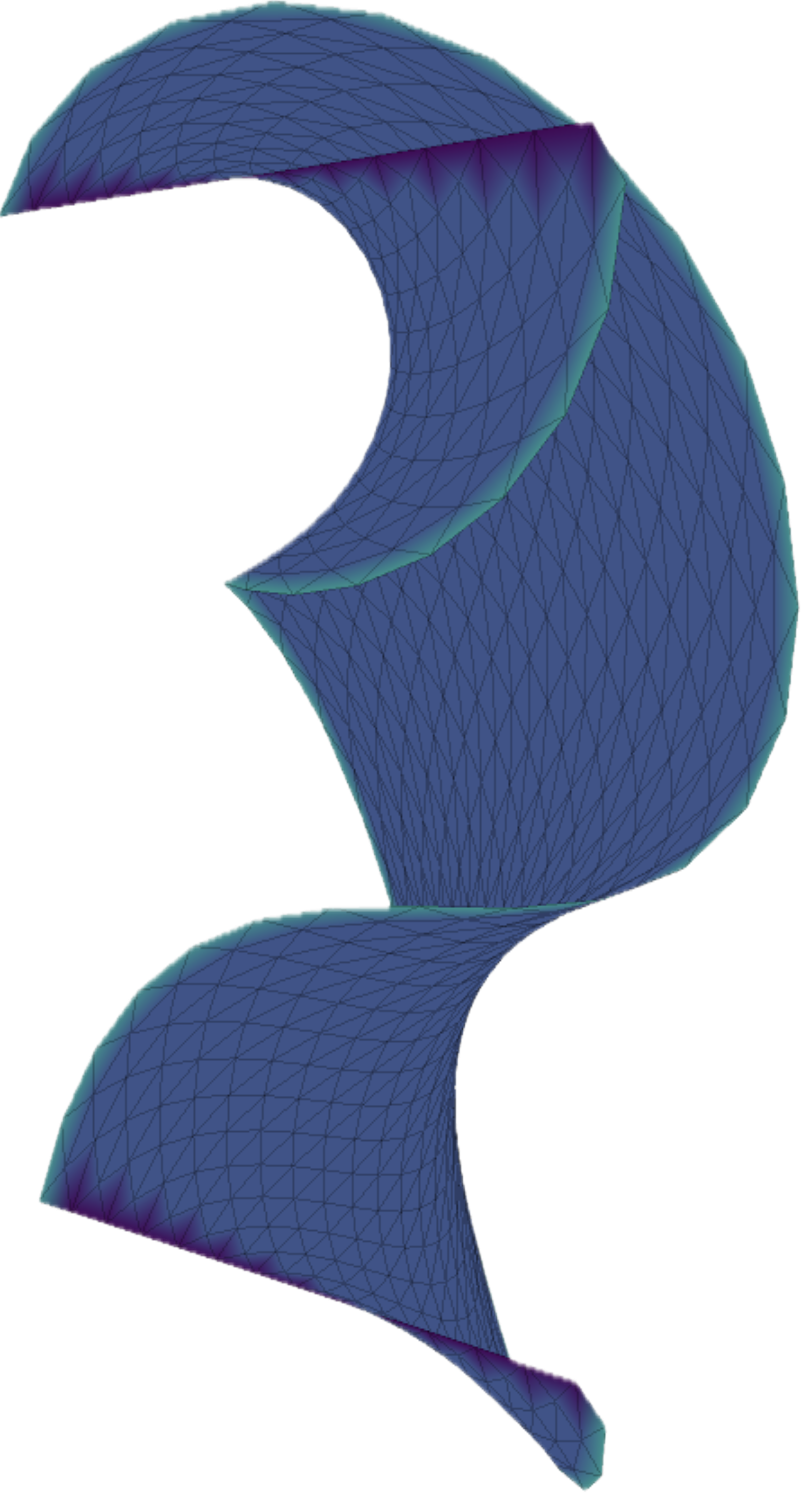
\includegraphics[width=0.8\columnwidth]{../images/helix_BC.png}\vspace*{-50mm}
    \hspace*{20mm}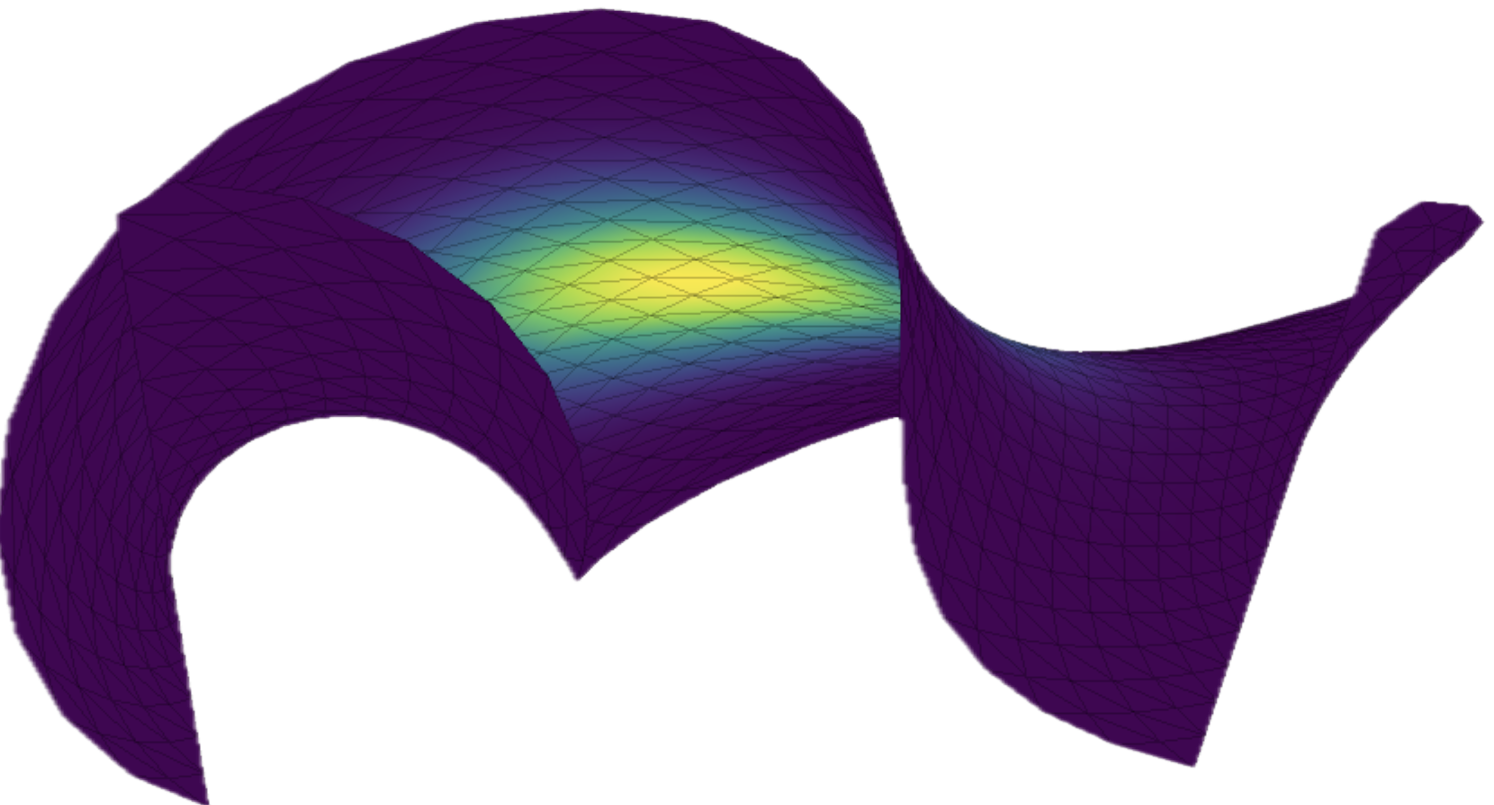
\includegraphics[width=0.8\columnwidth]{../images/helix_force.png}\vspace*{-50mm}
    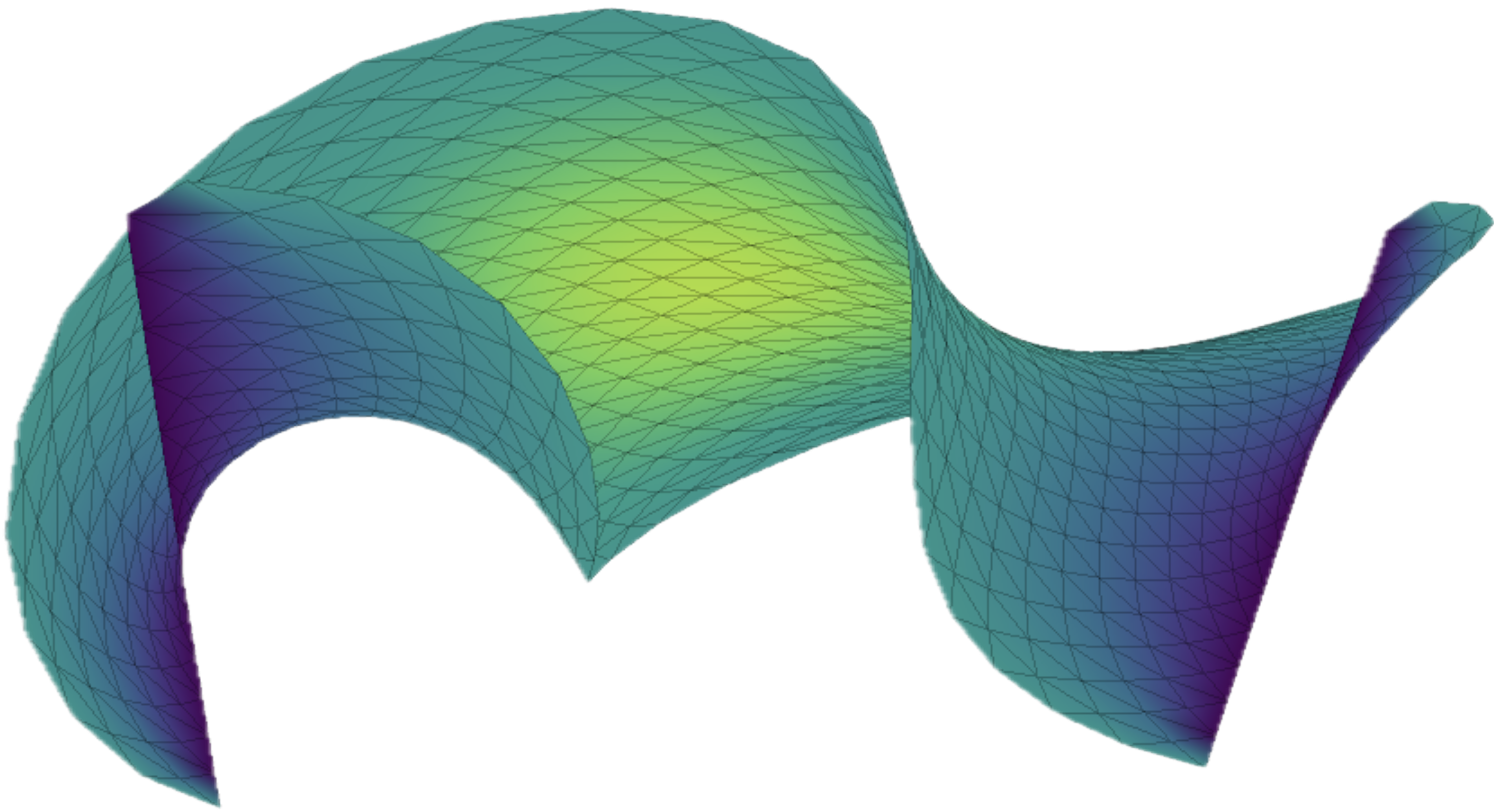
\includegraphics[width=0.8\columnwidth]{../images/helix_solution.png}%\vspace*{-50mm}
    \caption{}
    \label{fig:helix}
\end{figure}

\subsection*{Solving the Heat Equation}
As a demonstration, using the probabilistic solver, we solve the heat equation on the sphere, using the twice-integrated Wiener process. The speed of diffusion is linked to the Laplacians matrix $L$, which in turn depends on the scale of the geometry. We will therefore not give any units or specific values which are unimportant. See figure \ref{fig:heat_solution} for a demonsration of the solver. In figure can additionally get the joint distribution of the solution and show the uncertainties, see figure \ref{fig:heat_uncertainty}. We interpret the nonuniformity of the figure in the following way: The sphere mesh used has twelve\footnote{This mesh is created by using loop subdivision on the 12-tipped icosahedron with the \texttt{icosphere} Python package, which is a coarse approximation to the sphere geometry.} patches of vertices with incidence number 5 - in these, the solution is more certain than in the remaining ones. The Laplacian matrix will have five nonzero entries in the corresponding rows instead of six, and thus the solution here is less sensitive to the values of the neighbors. Additionally, the neighboring five vertices are spatially closer (the edge lengths are shorter), which introduces higher correlation between them.
\begin{figure}
    \centering
    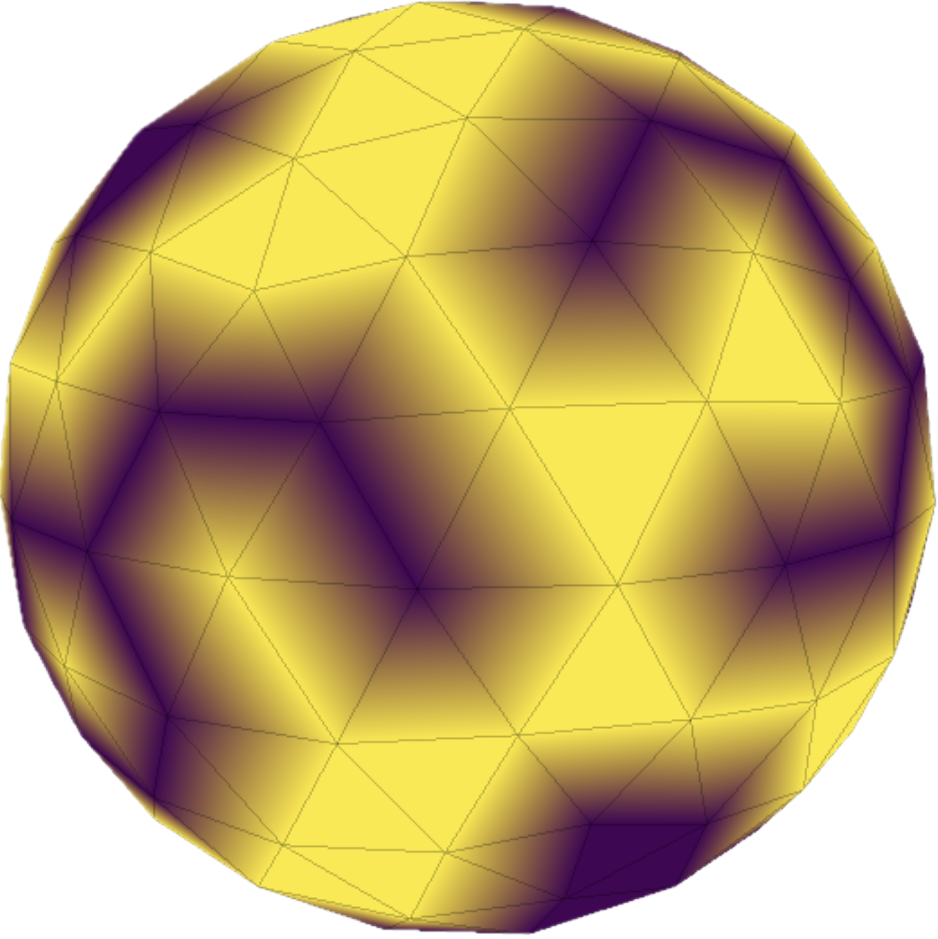
\includegraphics[width=0.9\columnwidth]{../images/sphere_entropic.png}\vspace*{3mm}
    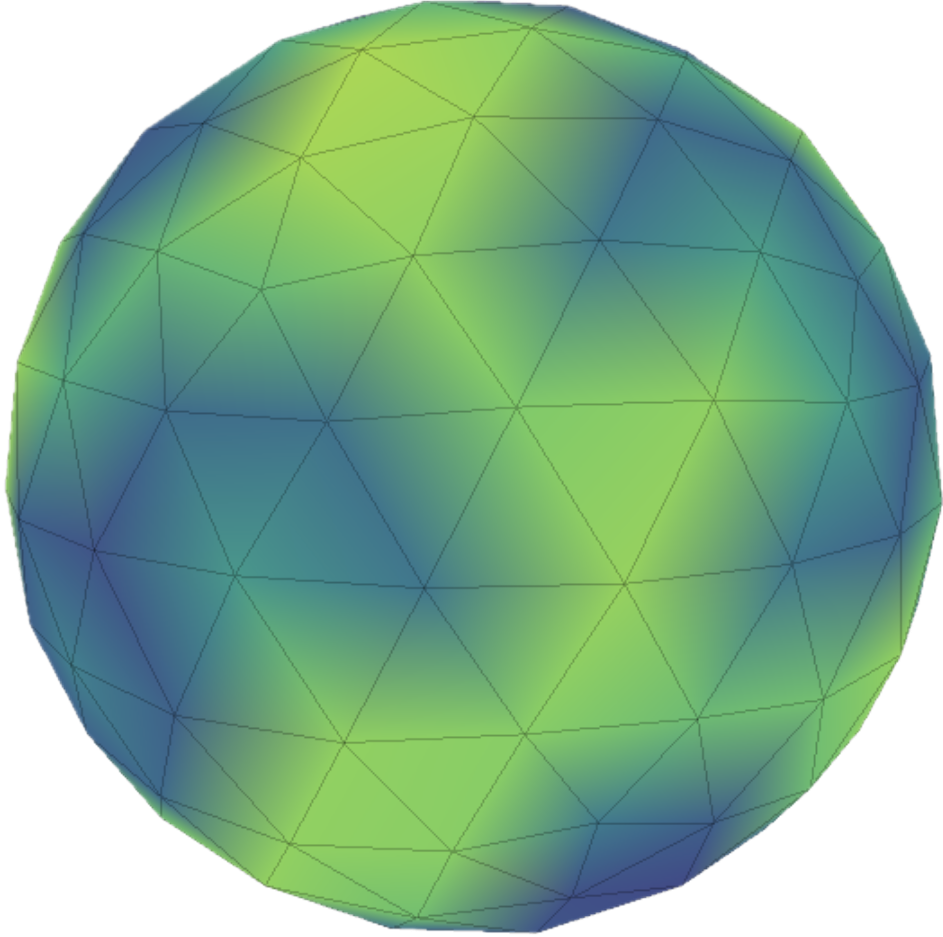
\includegraphics[width=0.9\columnwidth]{../images/sphere_smoothed.png}\vspace*{3mm}
    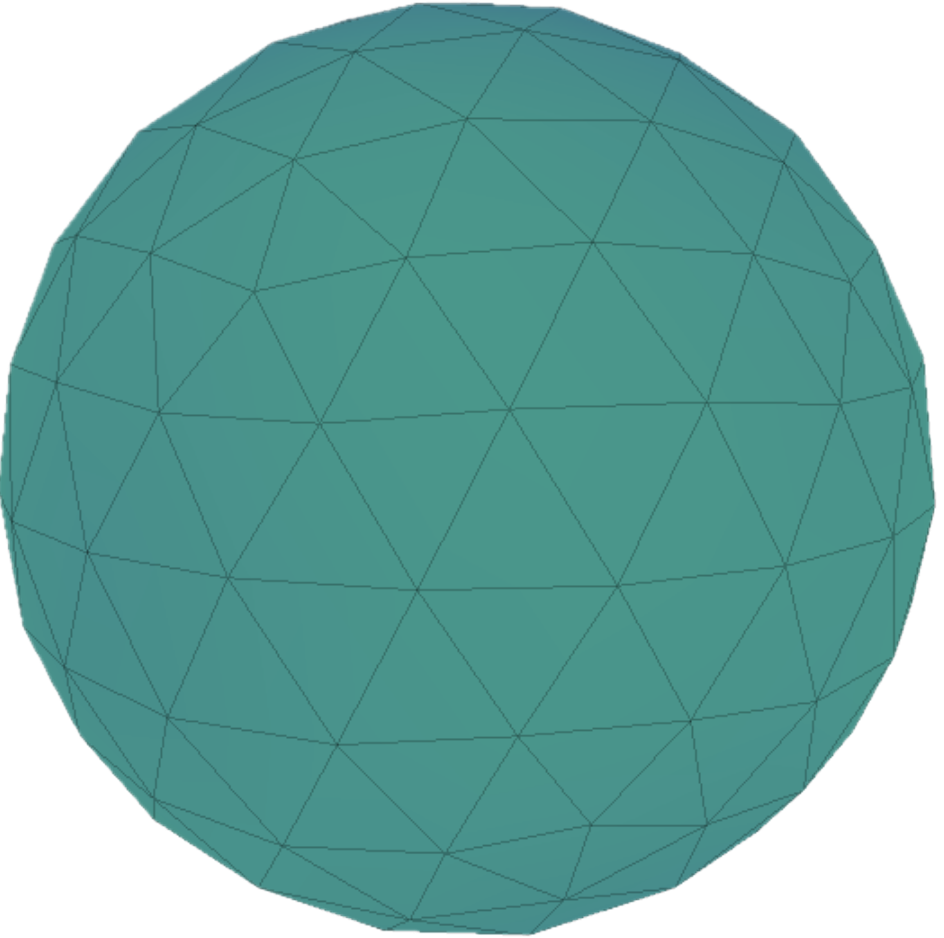
\includegraphics[width=0.9\columnwidth]{../images/sphere_cooled.png}\vspace*{3mm}
    \caption{The heat equation solved on the sphere. Uppermost image is the initial condition, where each vertex has been assigned to $\{-1, 1\}$ uniformly at random. Subsequent images are spaced equally apart in time, illustrating the heat diffusion. Yellows are positive temperatures, blues are negative temperatures.}
    \label{fig:heat_solution}
\end{figure}

\subsection*{The Laplacian captures the length-scale}
We visualize the Laplacian capturing length-scales on the Utah teapot \cite{utah} has been scaled so the body of the teapot is approximately a unit sphere. Figure \ref{fig:teapot_heat_solution} shows again the heat equation initial step and a short time later. The Utah teapot has highly non-uniform dual face areas, especially around the rim at the lid. As the diffusion process is not scale-invariant is illustrated by the fact that the temperature here will smooth out much quicker than in the remaining, bigger patches.
\begin{figure}
    \centering
    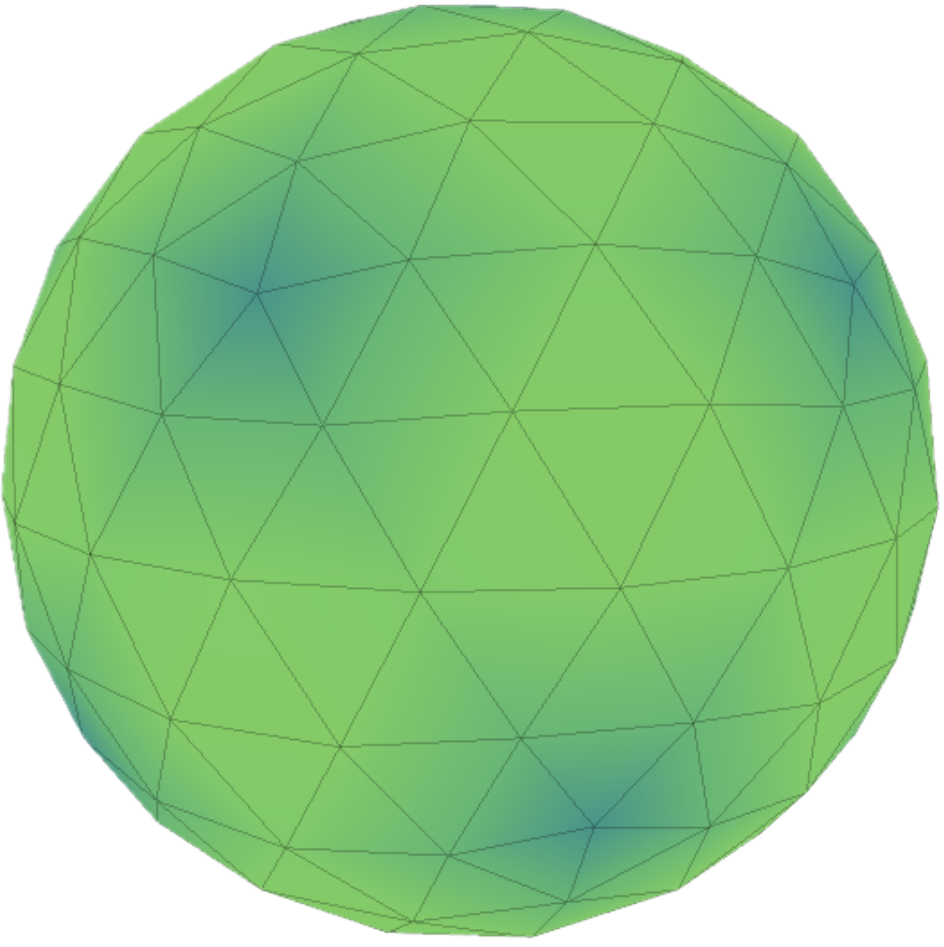
\includegraphics[width=0.9\columnwidth]{../images/sphere_uncertainty.png}\vspace*{3mm}
    \caption{The marginal standard deviations of the solution at the second step in figure \ref{fig:heat_solution}. Darker colors mean lower uncertainty. The uncertainty is miniscule and has been scaled up for illustration.}
    \label{fig:heat_uncertainty}
    \vspace*{10mm}
    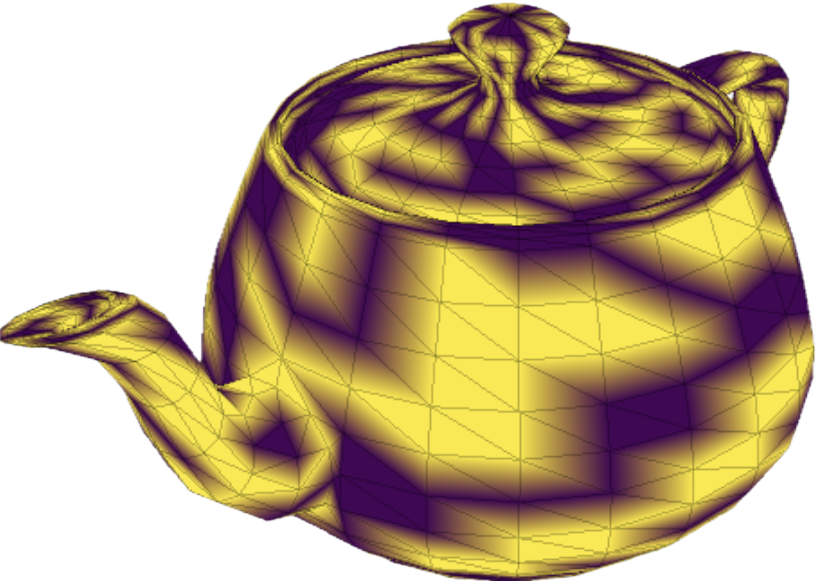
\includegraphics[width=0.9\columnwidth]{../images/teapot_entropic.png}\vspace*{3mm}
    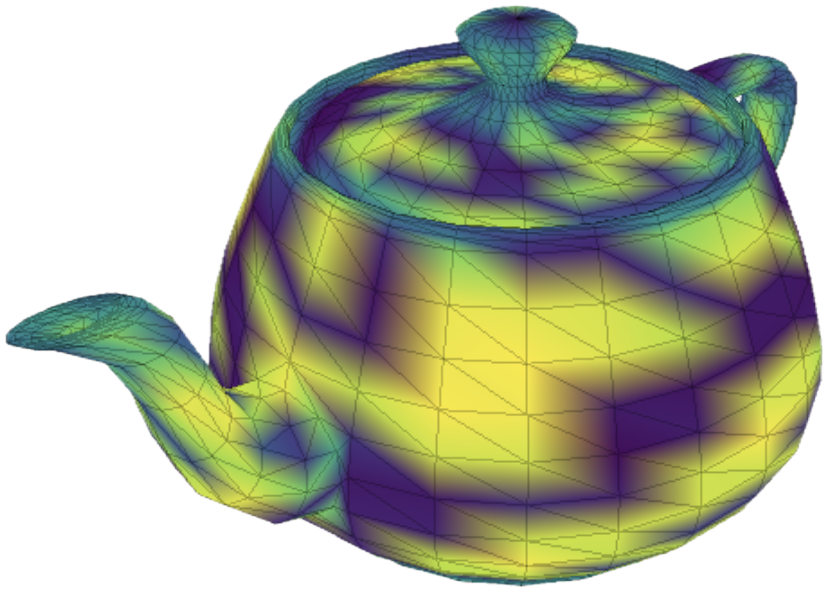
\includegraphics[width=0.9\columnwidth]{../images/teapot_smoothed.png}\vspace*{3mm}
    \caption{The heat equation solved on the Utah Teapot. The initial conditions are akin to the ones in fig. \ref{fig:heat_solution} and shown in the topmost figure. Below is the heat diffusion after a short time.}
    \label{fig:teapot_heat_solution}
\end{figure}

\subsection*{Solving the Wave Equation On an Intrinsically Triangulated Surface}
Using our algorithm from chapter \ref{sec:intrinsic_triangulation}, we use triangulate the bell-curve geometry, compute the Laplacian, and solve the wave equation on it. To motivate the expected behaviour, one can think of a wave as simply a shockwave traveling at constant speed from a source, which we visualize an approximation of in figure \ref{fig:dijkstra}. There are multiple ways to compute the location of the front of the shockwave, such as the ones proposed and compared in \cite{vector_dijkstra} and \cite{heat_method}. For the sake of ease of implementation, we use the simplest one, Dijkstra's single-source-all-paths algorithm. The figure shows level-sets of the distance function to the source (on the left, at coordinates $(-0.5, 0.0)$). This figure suggests that one should observe the wave traveling around the bump faster than across it, which is reasonable, given the detour the wave would take to travel across the bump.
This simplification ignores the reflections and interference that might occur due to our Dirichelet BCs (which are fixed at a wave-height of zero).
\\
In the four stacked figures in figure \ref{fig:bell_wave}, we show the solution of the wave equation on the bell-curve mesh.
\label{fig:bell_wave}

\begin{figure}
    \centering
    \hspace*{-6mm}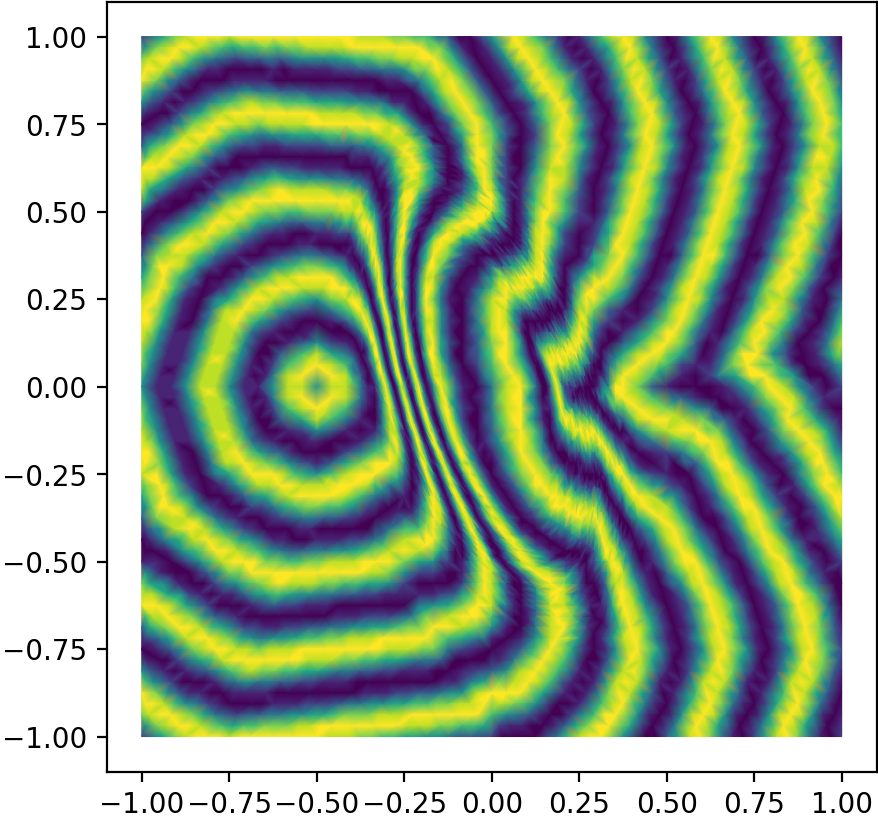
\includegraphics[width=0.9\columnwidth]{../images/bell_wave_distances.png
    }\vspace*{10mm}
    \caption{Level sets of the distance function from the left-of-centersource}
    \label{fig:dijkstra}
    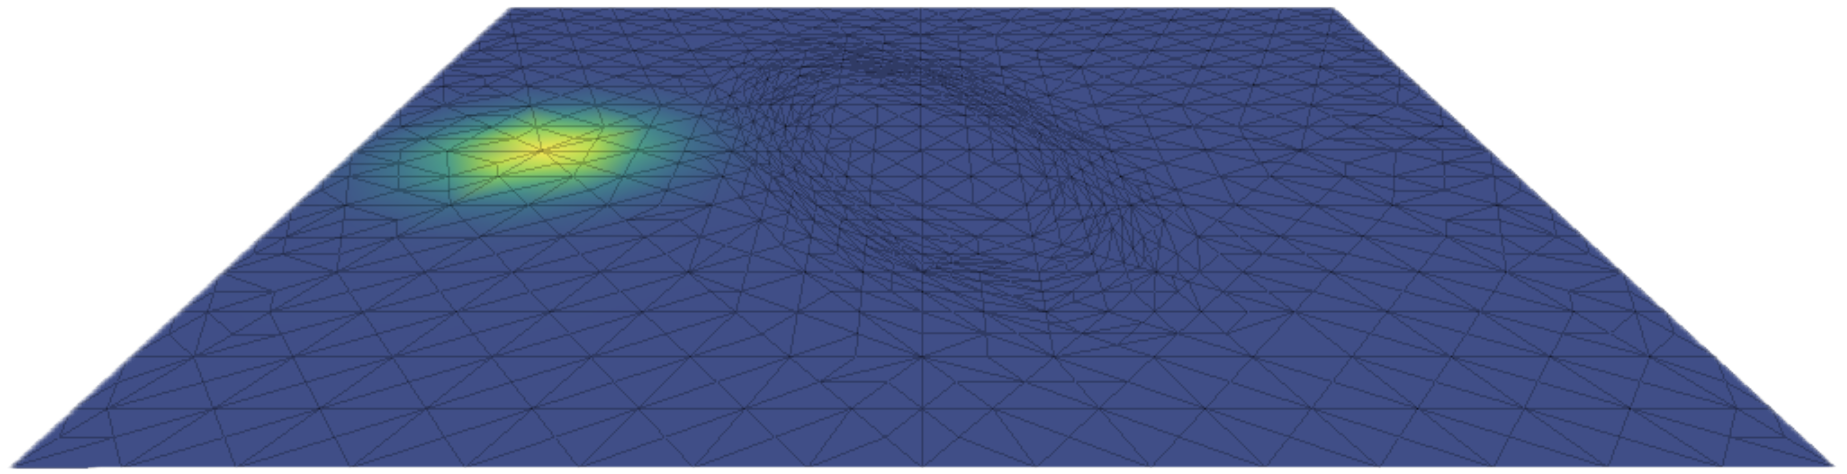
\includegraphics[width=0.9\columnwidth]{../images/bell_wave_0.png}\vspace*{3mm}
    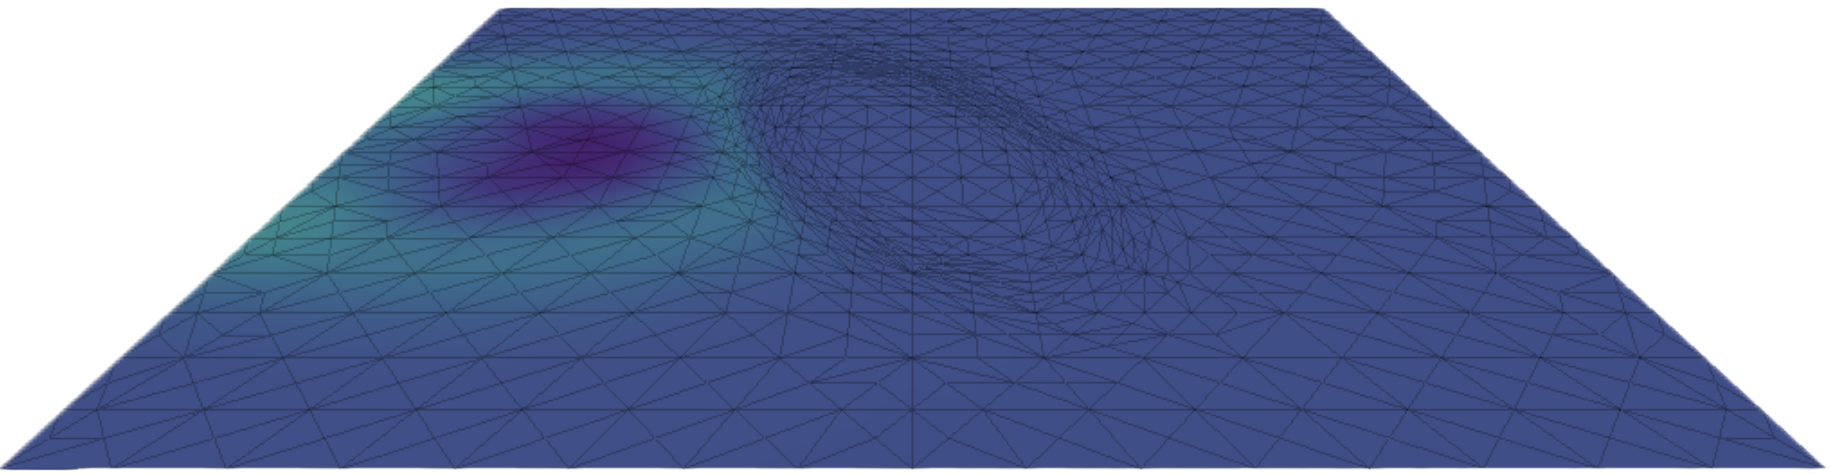
\includegraphics[width=0.9\columnwidth]{../images/bell_wave_1.png}\vspace*{3mm}
    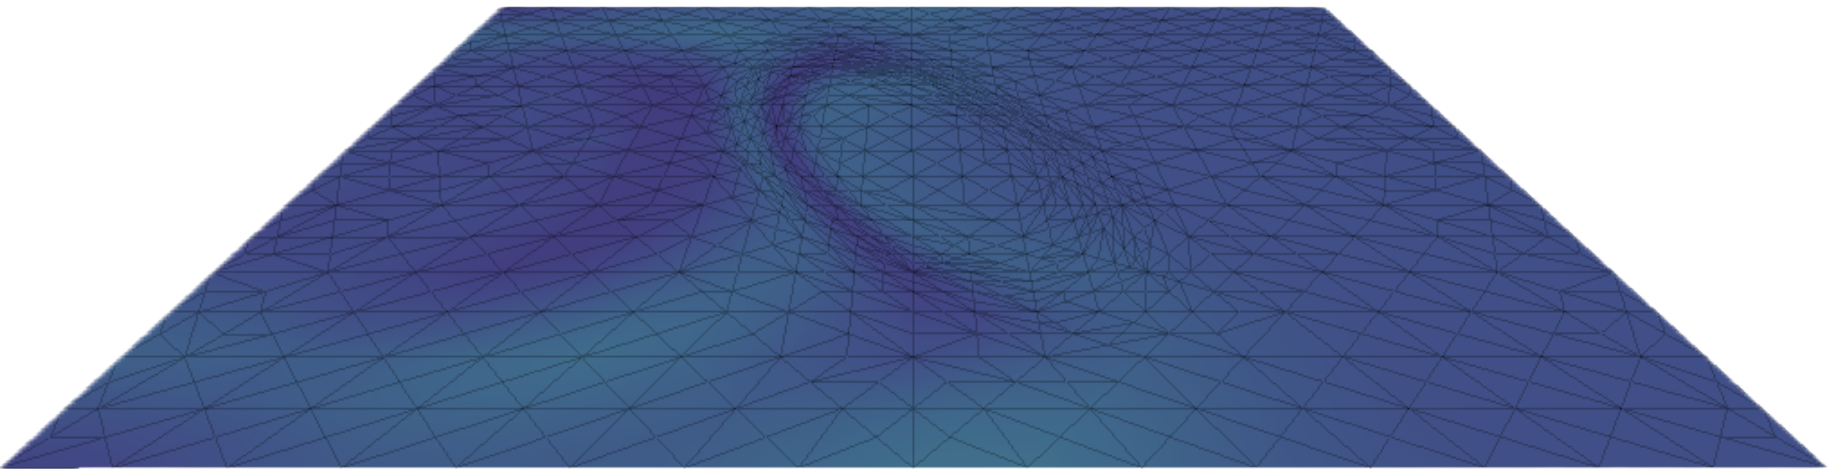
\includegraphics[width=0.9\columnwidth]{../images/bell_wave_2.png}\vspace*{3mm}
    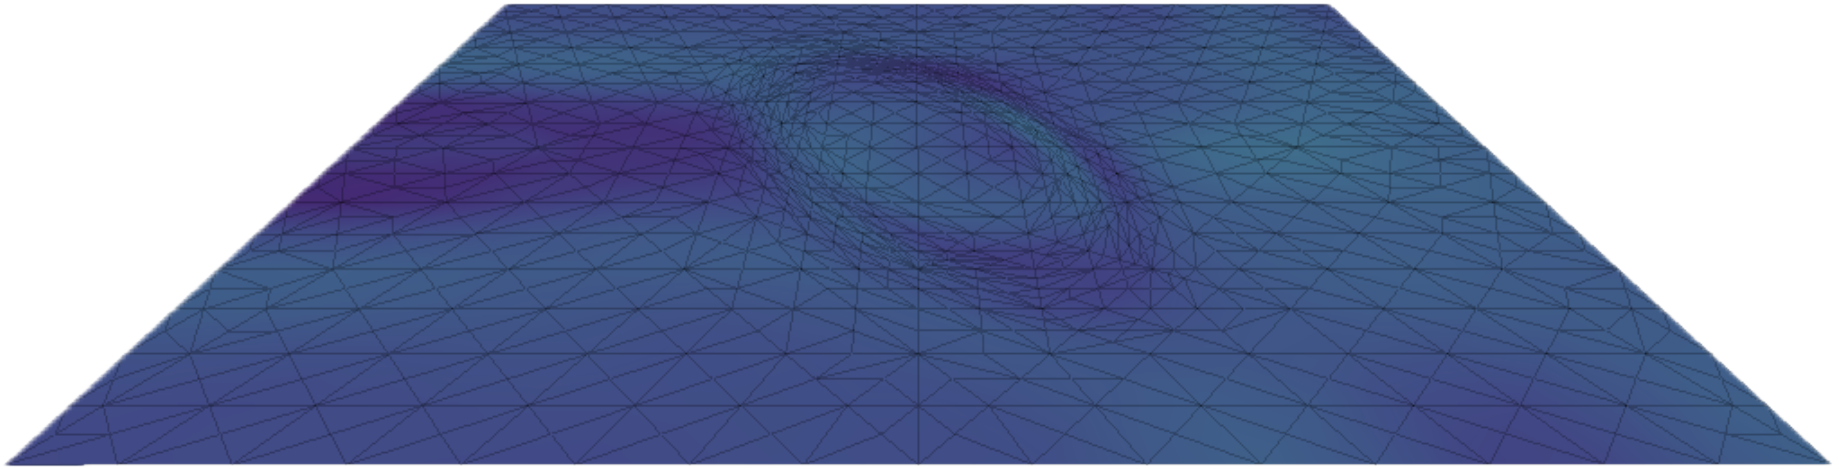
\includegraphics[width=0.9\columnwidth]{../images/bell_wave_3.png}\vspace*{3mm}
    \caption{.}
    \label{fig:bell_wave}
\end{figure}





\subsection*{Encoding Prior knowledge about an PDE into a LTI SDE}
This idea was adapted from \cite{exponential_probabilistic} in which the authors use integrated Ornstein-Uhlenbeck processes (chapter \ref{sec:prior}) to solve stiff ODEs. An example of a stiff ODE is 
$$\frac{du}{dt} = -20u + g(u)$$
where $g(u)$ is some nonlinear term in the vector field. The linear part of this ODE is the term $-20u$. This part can be solved exactly by the mean of an integrated Ornstein-Uhlenbeck process with rate-parameter $a=20$. Using such a prior leads to faster convergence than the usual integrated Wiener process, because it exactly solves the linear part of the ODE.
We will show that the same idea can be applied to PDEs and give another related prior process.
\\
\example{Mean of the Integrated Process is unaltered}{
Assume we have a prior process that we believe captures the dynamics of the ODE we want to solve. We will show that the process yielded by repeated integration will have the same mean, given suitable initial conditions. 
For a LTI SDE of the form \ref{eq:LSDE_definition} over scalar state-space $\vec{u}$, the matrix  will have this structure:
$$F^\prime = \begin{bmatrix}
    0 & 1 \\ -a & -b
\end{bmatrix}$$
This encodes dynamics of a damped spring-mass system, like we have seen in an example in both chapter \ref{sec:pde} and \ref{sec:prior}. The mean of this process at time $t$ is given by (using eq. \ref{eq:SDE_mean}):
\begin{align*}
    \mathbb{E}\left[\begin{pmatrix}
        \vec{u}_{0}(t) \\ \vec{u}_{1}(t)
    \end{pmatrix} \!\right] &= 
    e^{F^\prime t} \mathbb{E}\left[\begin{pmatrix}
        \vec{u}_{0}(0) \\ \vec{u}_{1}(0)
    \end{pmatrix} \!\right]
\end{align*}
$\vec{u}_0$, the solution function of the ODE encoded in $F^\prime$ is the mean.
\\
If we model it integrated once more, we get the following system dynamics matrix 
$$F^\prime = \begin{bmatrix}
    0 & 1 & 0 \\ 0 & 0 & 1 \\ 0 & -a & -b
\end{bmatrix}$$
This process will have mean given by (denoting the integral of $\vec{u}_0$ as $\vec{u}_{-1}$):
\begin{align*}
    \mathbb{E}\left[\begin{pmatrix}
        \vec{u}_{-1}(t) \\ \vec{u}_{0}(t) \\ \vec{u}_{1}(t)
    \end{pmatrix} \!\right] &= 
    e^{F^\prime t} \mathbb{E}\left[\begin{pmatrix}
        \vec{u}_{-1}(0) \\ \vec{u}_{0}(0) \\ \vec{u}_{1}(0)
    \end{pmatrix} \!\right]
\end{align*}

If we integrate it $q-1$ times, we get the following system dynamics matrix $F\in\reals^{q+1\times q+1}$

$$F = \begin{bmatrix}
    0 & 1 & 0 & \!\!\dots\!\! & 0 & 0 & 0 \\
    0 & 0 & 1 & \!\!\dots\!\! & 0 & 0 & 0 \\
    0 & 0 & 0 & \!\!\dots\!\! & 0 & 0 & 0 \\
    \vdots & \!\!\ddots\!\! & \!\!\ddots\!\! & \!\!\ddots\!\! & \!\!\ddots\!\! & \!\!\ddots\!\! & \vdots \\
    0 & 0 & 0 & \!\!\dots\!\! & 0 & 1 & 0 \\
    0 & 0 & 0 & \!\!\dots\!\! & 0 & 0 & 1 \\
    0 & 0 & 0 & \!\!\dots\!\! & 0 & \!\!-b & \!\!\!\!-a \\
\end{bmatrix}$$

$F$ encodes the ODE:
\begin{align}
    \frac{d}{dt}\vec{u}_0 &= \vec{u}_1 \nonumber
    \\\frac{d}{dt}\vec{u}_i &= \vec{u}_{i+1} \hspace{5mm} \i \in \{1, \dots, q\!-\!1\}\label{eq:relationship}
    \\\frac{d}{dt}\vec{u}_q &= -b\vec{u}_{q-2} - a\vec{u}_{q-1}\label{eq:to_integrate}
\end{align}
By taking the expectation of equation eq. \ref{eq:to_integrate} we can show that the mean of the $q$-times integrated process is the same as the mean of the original process.
\begin{align*}
    \mathbb{E}\left[\begin{pmatrix}
        \vec{u}_{q\!-\!1}(t) \\ \vec{u}_{q}(t)
    \end{pmatrix} \!\right] &= 
    e^{F^\prime t} \mathbb{E}\left[\begin{pmatrix}
        \vec{u}_{q}(0) \\ \vec{u}_{q\!-\!1}(0)
    \end{pmatrix} \!\right]
    \\
    &\hspace*{2mm}\rotatebox[origin=c]{90}{$\Leftrightarrow$}
    \\
    \int \mathbb{E}\left[\begin{pmatrix}
        \vec{u}_{q\!-\!1}(t) \\ \vec{u}_{q}(t)
    \end{pmatrix} \!\right] &= \int 
    e^{F^\prime t} \mathbb{E}\left[\begin{pmatrix}
        \vec{u}_{q}(0) \\ \vec{u}_{q\!-\!1}(0)
    \end{pmatrix} \!\right]
    \\
    &\hspace*{2mm}\rotatebox[origin=c]{90}{$\Leftrightarrow$}
    \\
    \int\!\!\!\!\int \mathbb{E}\left[\begin{pmatrix}
        \vec{u}_{q\!-\!1}(t) \\ \vec{u}_{q}(t)
    \end{pmatrix} \!\right] &= \int\!\!\!\!\int 
    e^{F^\prime t} \mathbb{E}\left[\begin{pmatrix}
        \vec{u}_{q}(0) \\ \vec{u}_{q\!-\!1}(0)
    \end{pmatrix} \!\right]
    \\
    &\hspace*{2mm}\rotatebox[origin=c]{90}{$\Leftrightarrow$}
    \\
    \underbrace{\int\!\!\!\dots\!\!\!\int}_{\times\! (q-\!1)} \mathbb{E}\left[\begin{pmatrix}
        \vec{u}_{q\!-\!1}(t) \\ \vec{u}_{q}(t)
    \end{pmatrix} \!\right] &= \underbrace{\int\!\!\!\dots\!\!\!\int}_{\times\! (q-\!1)} 
    e^{F^\prime t} \mathbb{E}\left[\begin{pmatrix}
        \vec{u}_{q}(0) \\ \vec{u}_{q\!-\!1}(0)
    \end{pmatrix} \!\right]
    \\
    &\hspace*{2mm}\rotatebox[origin=c]{90}{$\Leftrightarrow$} \text{  (linearity of integral)}
    \\
    \mathbb{E}\left[\begin{pmatrix}
        \vec{u}_{0}(t) \\ \vec{u}_{1}(t)
    \end{pmatrix} \!\right] &= 
    e^{F^\prime t} \mathbb{E}\left[\begin{pmatrix}
        \vec{u}_{0}(0) \\ \vec{u}_{1}(0)
    \end{pmatrix} \!\right]
\end{align*}
}

\definition{Wave Process}{
    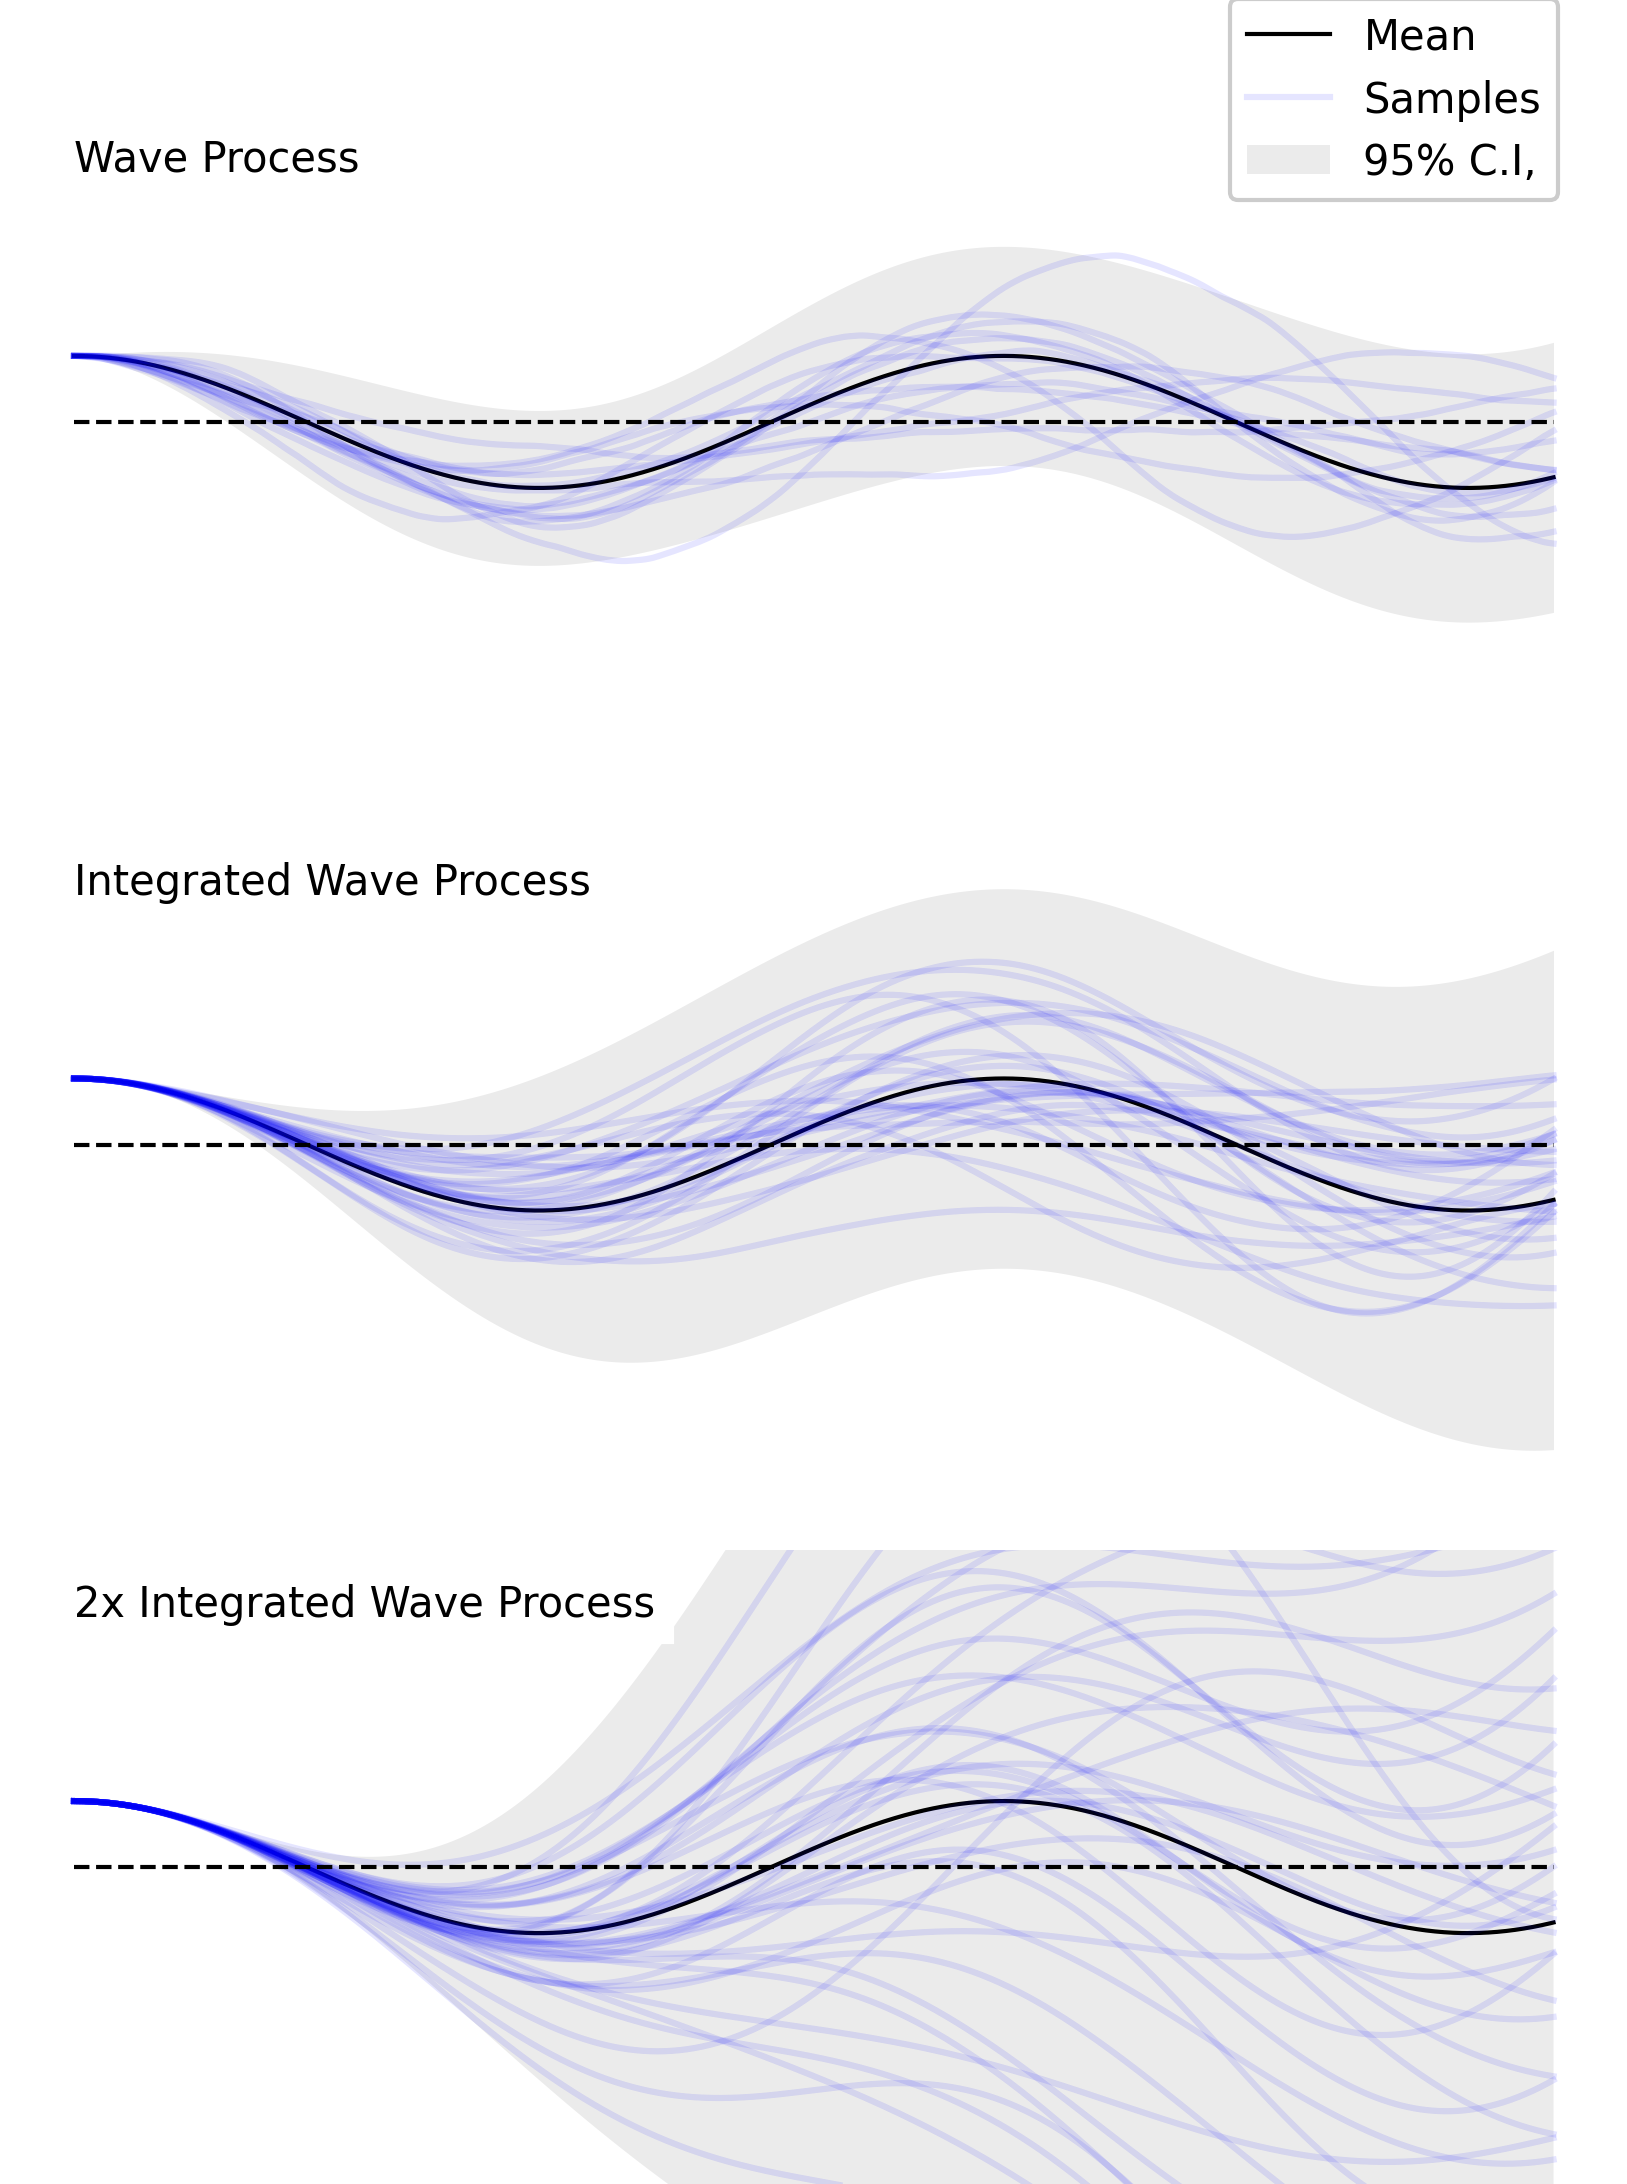
\includegraphics[width=\columnwidth]{../images/wave_process.png}
    \captionof{figure}{Iterated integrations of the Wave Process.}
    \label{fig:wave_process}
    This process really is an instance of the Ornstein Uhlenbeck Process mention in chapter \ref{sec:prior}, but for our purposes it will be more descriptive to refer to it as a "Wave process". 
    \\
    It however already has the wave-like behaviour at $q=1$, which is shown in the first slide in figure \ref{fig:wave_process}. The second slide shows the behaviour at $q=2$ and the third slide shows the behaviour at $q=3$. 
    \\
    Since we need at least $q=2$ derivatives for a prior process to be applicable for second order ODEs, we will never work with the Wave process itself, but only with its iterated integrations.
   
    The Wave process is defined by the following state-space representation:
    $$F=\begin{bmatrix}
        0 & 1 \\ -a & 0
    \end{bmatrix} \hspace{1cm} L=\begin{bmatrix}
        0 \\ 
        1 
    \end{bmatrix}$$
    \\ The Twice Integrated Wiener Process has 3-dimensional state-space with $$F=\begin{bmatrix}
        0 & 1 & 0 \\ 0 & 0 & 1 \\ 0 & -a & 0
    \end{bmatrix} \hspace{1cm} L=\begin{bmatrix}
        0 \\ 0 \\ 1
    \end{bmatrix}$$
    \\ The posterior means of the $q$-times integrated Wiener process are 2q + 1-ic splines (\cite{probnum}) - see the figure above. There is in principle nothing preventing us from using higher order integrated Wiener processes, but numerical issues can be encountered already at $q=3$. We will tackle this later.
}
\newpage
In this section we will apply the solver and our built Laplace-matrices to some ODEs. We will investigate how different choices of prior processes can give an inductive bias to the solver, helping it solve the ODE more exactly.
We will use a similar idea, but instead of using integrated Ornstein-Uhlenbeck processes, we will use the Laplacian matrices we have built in earlier sections to build PDE priors taylored to different kind of problems.
\subsection*{Physically Informed Priors}
As problems, we choose a nonlinear version of the heat and wave equation, with varying degrees of nonlinearity. 
\begin{align}
    \frac{\partial}{\partial t}u = -\Delta u - au^2\label{eq:nonlinear_heat}
\end{align}
\begin{align}
    \frac{\partial^2}{\partial t^2}u = -\Delta u - a\tan u\label{eq:nonlinear_wave}
\end{align}
The hypothesis is that, for small nonlinearities, a prior that encodes the linear heat/wave dynamics will outperform the integrated Wiener process. As the nonlinearities become larger and we move away from the linear dynamics, the prior will not as related and we should expect a decrease in efficiency.  We run both problems for $a\in\{0, 10^{-3}, 1\}$.
\\ For eq. \ref{eq:nonlinear_wave}, we will use integrated Wave processes as our prior, and for eq. \ref{eq:nonlinear_wave} we will use the Heat process. We will compare against repeatedly integrated Wiener processes as priors.
\\\\
The problems will be solved on the 2D surface of the sphere, approximated by a 12-vertex icosphere. The vector fields are integrated from $t_0=0$ to $t_{\mathbb{T}}=10$.  We will grade the PN solutions by the root-mean-square-error at all computed timesteps against a high-accuracy reference solution implemented in \texttt{diffrax} \cite{diffrax}, using the Kvaerno5/4 method \cite{kvaerno}, suitable for stiff problems like the heat and wave equation. The reference solution has both relative and absolute tolerances of $10^{-8}$, which then also serves as a lower bound for the error of the PN solution.
\\ The PN solution will be computed for varying amount of timesteps and for different choices of $q$ in the prior process. We will then plot the work/precision diagrams for the different choices of $q$ and $a$.
\subsection*{Results}
See figures \ref{fig:heat} through \ref{fig:wave big} for all work/precision diagrams. In the figures, the integrated wiener process is depicted in green, the integrated wave process in blue, and the integrated heat process in red. The x-axis shows the number of timesteps, and the y-axis shows the root-mean-square-error. As the number of steps increase, the error generally decreases. For increasing $q$, the error drops faster.
\\ The integrated Wiener processes are generally being outperformed, however less decisively so for significant nonlinearities ($a = 1$). For $a=0$ the expected exact solution of the priors is observed, even for $10$ timesteps, massively outperforming the integrated Wiener process (but this was not a fair competition).
\\ The result confirm that an appropriate prior process gives the solver an inductive bias that helps solve the ODEs more exactly and efficiently.s
\begin{figure}
    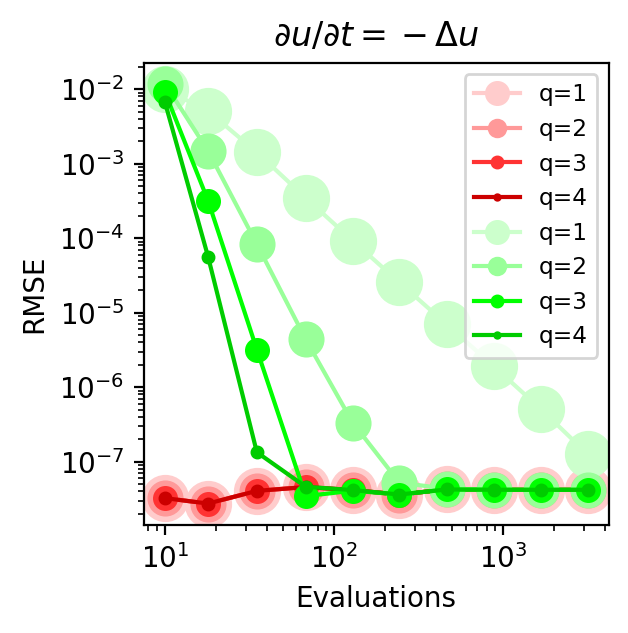
\includegraphics[width=\columnwidth]{../images/solver_heat.png}
    \caption{}
    \label{fig:heat}
    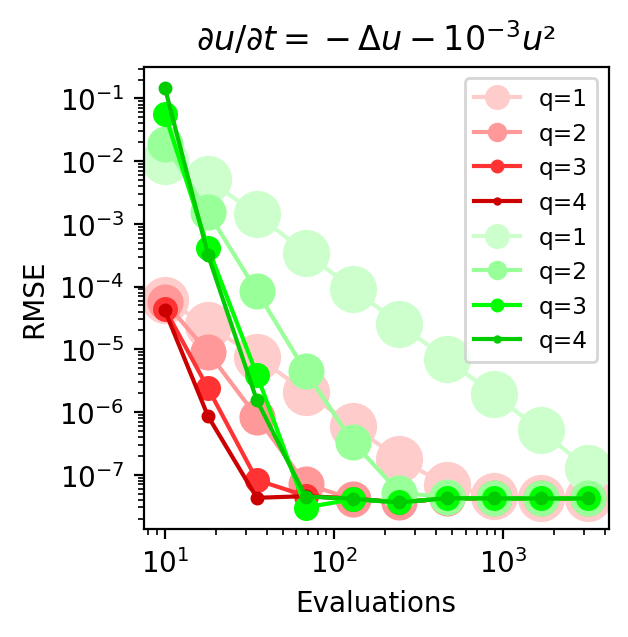
\includegraphics[width=\columnwidth]{../images/solver_heat and medium square.png}
    \caption{}
    \label{fig:heat medium}
    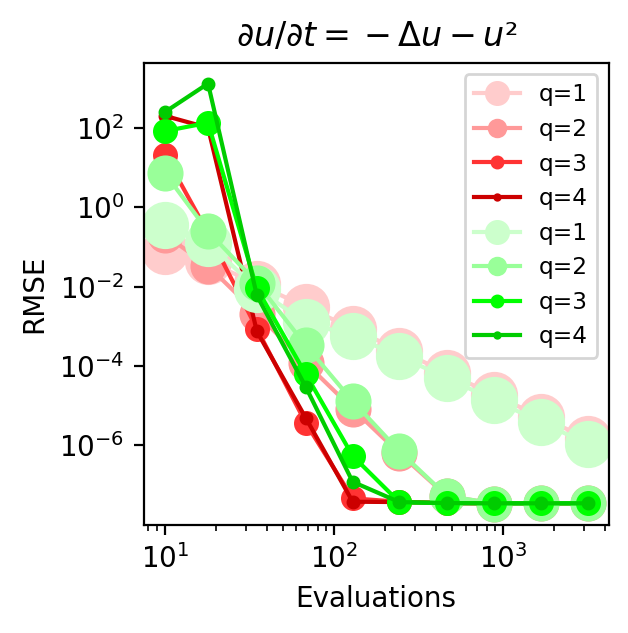
\includegraphics[width=\columnwidth]{../images/solver_heat and big square.png}
    \caption{}
    \label{fig:heat big}
\end{figure}
\begin{figure}
    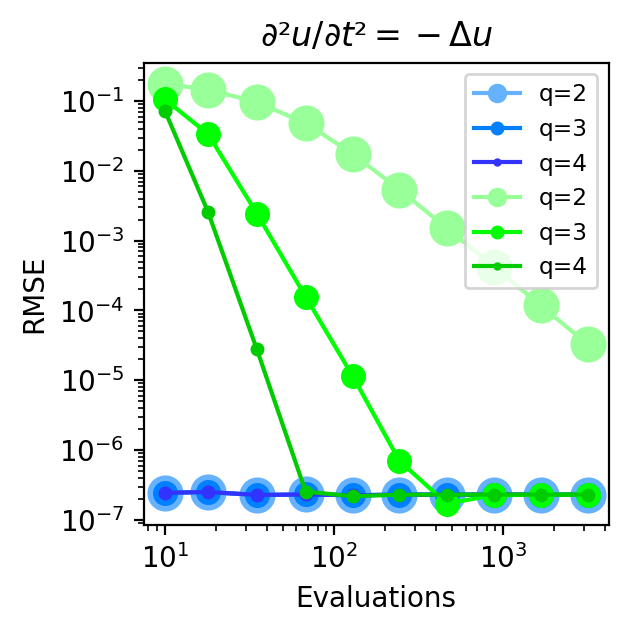
\includegraphics[width=\columnwidth]{../images/solver_wave.png}
    \caption{}
    \label{fig:wave}
    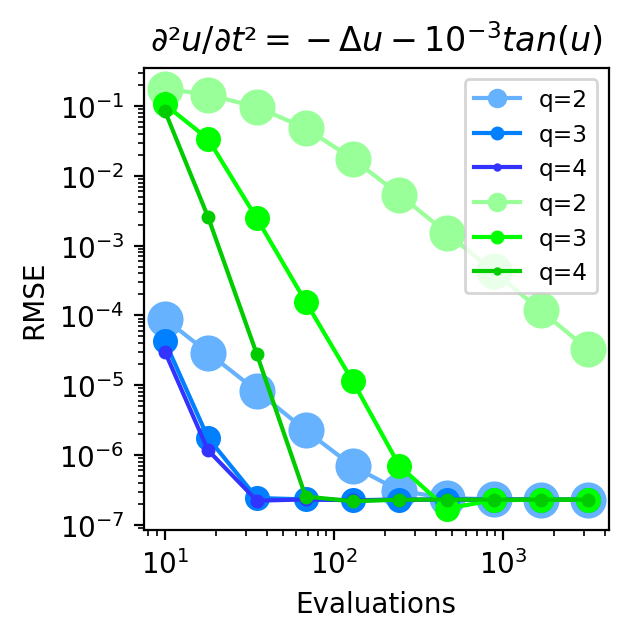
\includegraphics[width=\columnwidth]{../images/solver_wave and medium tan.png}
    \caption{}
    \label{fig:wave medium}
    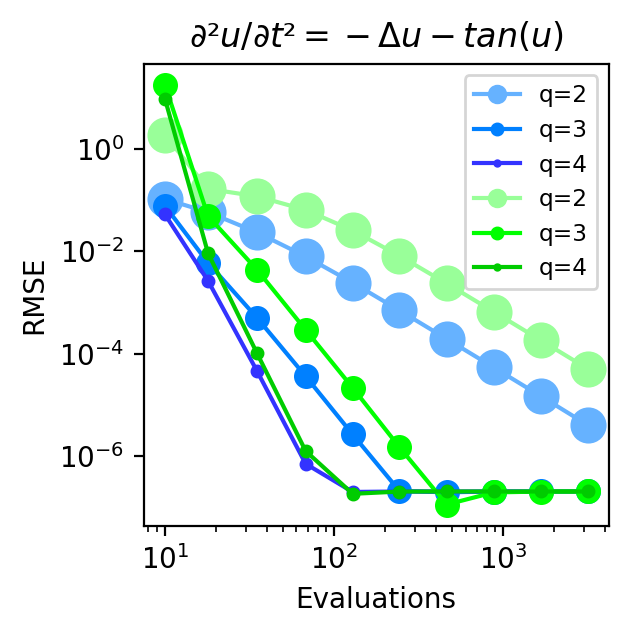
\includegraphics[width=\columnwidth]{../images/solver_wave and big tan.png}
    \caption{}
    \label{fig:wave big}
\end{figure}


\ifdefined\COMPILINGFROMMAIN
\else    
    \end{document}
\fi